
\section{Formulas}

\subsection{Relación entre rotación, frecuencia y número de pares de polos en máquinas síncronas.}

\begin{equation}
n= \frac{60 \cdot f}{p}     
\end{equation}
\begin{equation}
f= \frac{n \cdot p}{60}     
\end{equation}
\begin{equation}
p= \frac{60 \cdot f}{n}     
\end{equation}


siendo:

$f$:frecuencia en Herz(Hz)

$n$:Velocidad de rotación ( en RPM:revoluciones por minuto)

$p$:Número de pares de polos. 


\subsection{Triángulo de Potencia}


\begin{figure}[h]
    \centering
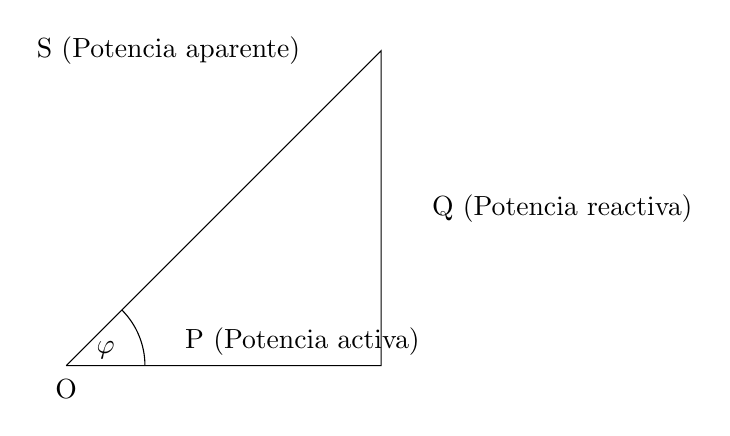
\begin{tikzpicture}

\draw (0,0) -- (4,0) -- (4,4) -- (0,0);
\node (O) at (0,-0.3) {O};
\node (P) at (3,0.3) {P (Potencia activa)};
\node (Q) at (6.3,2) {Q (Potencia reactiva)};
\node (S) at (1.3,4) {S (Potencia aparente)};
\node (phi) at (0.5,0.2) {$\varphi$};
\draw (1,0) arc (0:45:1cm);
\end{tikzpicture}

    \caption{Triángulo de potencia.}
    \label{fig:my_label}
\end{figure}


\begin{center}
\begin{table}[h]
\centering
    \begin{tabular}{|r|c|c|}\hline
Descripción & Fórmula & Unidad SI\\\hline
Potencia Activa & $P=V I cos(\varphi)$ & Watt(W)\\
Potencia Reactiva & $Q=V I sen(\varphi)$ & Volt-Ampere Reactivo (VAr)\\
Potencia Aparente & $S=V I$ & Volt-Ampere (VA)\\ \hline
Impedancia &$Z^2=(X_L-X_C)^2+R^2$ & Ohm ($\Omega$)\\
Reactancia Inductiva & $X_L=2 \pi f L$ & Ohm($\Omega$)\\
Reactancia Capacitiva & $X_C=\frac{1}{2 \pi f C} $ & Ohm ($\Omega$)\\\hline
Caballo de Vapor & $1CV = 736W$& CV (siempre es potencia activa) \\
Caballo de Fuerza & $1HP = 746W$& HP (siempre es potencia activa) \\ \hline
Resist. equiv. paralelo & $R_E = \frac{1}{\frac{1}{R_1}+\frac{1}{R_2}+...+\frac{1}{R_N}}$&
Ohm($\Omega$) \\
Resist.equiv. serie & $R_E = R_1+R_2+...+R_N$&
Ohm($\Omega$) \\ \hline

    \end{tabular}
    \caption{Fórmulas y unidades en Sistema Internacional.}
    \label{tab:my_label}
\end{table}
\end{center}


\newpage
\subsection{ Relación de tensiones en sistema trifásico equilibrado}

\begin{equation}
    V_c= \sqrt{3} \cdot V_s
\end{equation}

Siendo:

$V_c$: Tensión entre fases (tensión compuesta). 

$V_s$: Tensión entre fase y neutro (tensión simple). 


\subsection{Potencia en sistema trifasico}

\begin{equation}
    S= 3 \cdot  V_s \cdot I_s
\end{equation}
\begin{equation}
    P= 3 \cdot  V_s \cdot I_s \cdot cos(\varphi)
\end{equation}
\begin{equation}
    Q= 3 \cdot  V_s \cdot I_s \cdot sen(\varphi)
\end{equation}


\begin{equation}
    S= \sqrt{3} \cdot  V_c  \cdot I_s 
\end{equation}
\begin{equation}
    P= \sqrt{3} \cdot  V_c  \cdot I_s \cdot cos(\varphi)
\end{equation}
\begin{equation}
    Q= \sqrt{3} \cdot  V_c  \cdot I_s \cdot sen(\varphi)
\end{equation}



\begin{equation}
    P= S \cdot cos(\varphi)
\end{equation}
\begin{equation}
    Q= S \cdot sen(\varphi)
\end{equation}
\begin{equation}
\varphi=arctg({\frac{P}{Q}})
\end{equation}


